\documentclass[aspectratio=169, 10pt]{beamer}

\usetheme{Madrid}
\usecolortheme{whale}
\definecolor{mainblue}{RGB}{0,73,144}
\definecolor{accentred}{RGB}{180,30,40}
\definecolor{softgreen}{RGB}{34,139,34}
\definecolor{lightyellow}{RGB}{255,255,224}
\definecolor{lightgray}{RGB}{240,240,240}
\definecolor{oursgreen}{RGB}{232,245,233}
\definecolor{newbg}{RGB}{255,248,220}
\setbeamercolor{structure}{fg=mainblue}
\setbeamercolor{alerted text}{fg=accentred}
\setbeamercolor{block title}{bg=mainblue, fg=white}
\setbeamercolor{block body}{bg=lightgray}
\setbeamertemplate{navigation symbols}{}
\setbeamertemplate{footline}[frame number]
\setlength{\parskip}{0pt}

\usepackage[utf8]{inputenc}
\usepackage[T1]{fontenc}
\usepackage{amsmath, amssymb, amsfonts}
\usepackage{booktabs}
\usepackage{graphicx}
\usepackage{tikz}
\usetikzlibrary{arrows.meta, positioning, shapes, calc, decorations.pathreplacing, fit}
\usepackage{multirow}
\usepackage{hyperref}
\usepackage{fontawesome5}
\usepackage{pifont}
\usepackage{colortbl}

\title[AI Code Detection --- Progress Report]{%
  \textbf{Progress Report: AI-Generated Code Detection\\
  New Experiments, Methods \& Insights}}
\subtitle{Update for Advisor Meeting --- April 2026}
\author{%
  Dao Sy Duy Minh, Huynh Trung Kiet, Tran Chi Nguyen\\
  \textbf{HCMUS\_TheFangs}}
\institute{Ho Chi Minh City University of Science (HCMUS)\\VNUHCM}
\date{\today}

\begin{document}

\begin{frame}
\titlepage
\end{frame}

\begin{frame}{Outline --- What's New}
\tableofcontents
\end{frame}


% ════════════════════════════════════════════════════════════════════════
\section{New SOTA: DeTeCtiveCode (Exp27)}
% ════════════════════════════════════════════════════════════════════════

\begin{frame}{DeTeCtiveCode --- New Best Method (Author F1 = 71.53)}
\vspace{-0.2cm}
\begin{columns}[T]
\column{0.52\textwidth}
\begin{block}{Architecture: HierTree + SupCon + kNN}
\small
\begin{enumerate}\setlength\itemsep{3pt}
    \item[\faCogs] \textbf{Backbone:} SpectralCode (ModernBERT + AST + Struct + FFT)
    \item[\faProjectDiagram] \textbf{HierTree:} Family-aware affinity loss (from Exp18)
    \item[\faStar] \textbf{NEW: Multi-level SupCon} on both neural \& spectral projection heads (DeTeCtive, NeurIPS 2024)
    \item[\faSearch] \textbf{NEW: kNN blend} at test time ($k\!=\!32$, $\alpha\!=\!0.25$, bank $=$ 50K)
\end{enumerate}
\end{block}

\begin{exampleblock}{\scriptsize Loss Function}
\scriptsize
$\mathcal{L} = \mathcal{L}_{\text{task}} + 0.3\mathcal{L}_n + 0.3\mathcal{L}_s + \lambda_{\text{hier}}\mathcal{L}_{\text{hier}} + \lambda_{\text{sc}}\frac{\text{SupCon}_n + \text{SupCon}_s}{2}$
\end{exampleblock}

\column{0.46\textwidth}
\begin{alertblock}{Results (CoDET-M4)}
\centering\footnotesize
\begin{tabular}{lcc}
\toprule
& \textbf{F1} & $\boldsymbol{\Delta}$ vs UniX \\
\midrule
UniXcoder (paper) & 66.33 & --- \\
SpectralCode & 69.82 & +3.49 \\
HierTreeCode & 70.55 & +4.22 \\
\rowcolor{oursgreen}
\textbf{DeTeCtiveCode} & \textbf{71.53} & \textbf{+5.20} \\
\bottomrule
\end{tabular}
\end{alertblock}

\begin{block}{\scriptsize Per-Class Gains}
\scriptsize
\begin{tabular}{lccc}
\toprule
Human & GPT & Llama & CodeLlama \\
\midrule
0.986 & \textbf{0.780} $\uparrow$ & 0.825 & 0.745 \\
\bottomrule
\end{tabular}\\[2pt]
\begin{tabular}{lcc}
\toprule
\alert{Nxcode} & \alert{Qwen1.5} & GH source \\
\midrule
0.466 & \textbf{0.490} & \textbf{0.576} $\uparrow$ \\
\bottomrule
\end{tabular}
\end{block}
\end{columns}
\end{frame}


% ════════════════════════════════════════════════════════════════════════
\section{CoDET-M4: 22 Methods Explored}
% ════════════════════════════════════════════════════════════════════════

\begin{frame}{CoDET-M4: Full Leaderboard --- 22 Methods Ranked}
\vspace{-0.25cm}
\begin{columns}[T]
\column{0.52\textwidth}
\begin{block}{Top-12 by Author 6-Class Macro-F1}
\centering\scriptsize
\begin{tabular}{clcl}
\toprule
\textbf{\#} & \textbf{Method} & \textbf{F1} & \textbf{Key Idea} \\
\midrule
\rowcolor{oursgreen}
1 & \textbf{DeTeCtiveCode} & \textbf{71.53} & HierTree+SupCon+kNN \\
2 & HierTreeCode & 70.55 & Family-tree loss \\
3 & RAGDetect & 70.46 & Retrieval-augmented \\
\rowcolor{newbg}
4 & \textbf{HyperCode} & \textbf{70.33} & Hypernetwork head \\
\rowcolor{newbg}
5 & \textbf{KANCode} & \textbf{70.30} & B-spline KAN head \\
\rowcolor{newbg}
6 & \textbf{EnergyCode} & \textbf{70.26} & Energy-margin OOD \\
7 & BiScopeCode & 70.20 & MLM probe stream \\
8 & TTACode & 70.20 & Test-time adapt \\
9 & MultiGranCode & 70.19 & CharCNN fusion \\
10 & GroupDRO & 70.17 & Worst-group opt \\
\rowcolor{newbg}
11 & \textbf{WaveCLCode} & \textbf{70.16} & Wavelet contrastive \\
12 & SelfDistillCode & 70.14 & EMA distillation \\
\bottomrule
\end{tabular}
{\tiny \colorbox{newbg}{Yellow} = NEW since last report}
\end{block}

\column{0.46\textwidth}
\begin{block}{Bottom Methods + Failures}
\centering\scriptsize
\begin{tabular}{clcc}
\toprule
\textbf{\#} & \textbf{Method} & \textbf{F1} & \textbf{Note} \\
\midrule
13 & ProtoCon & 70.13 & Prototype bank \\
14 & MoECode & 70.04 & Sparse MoE \\
\rowcolor{newbg}
15 & \textbf{TTLCode} & \textbf{70.04} & Test-time LoRA \\
\rowcolor{newbg}
16 & \textbf{IBCode} & \textbf{70.02} & Info bottleneck \\
\rowcolor{newbg}
17 & \textbf{MambaCode} & \textbf{69.98} & Selective SSM \\
18 & SpectralCode & 69.82 & FFT spectral \\
19 & GraphStyleCode & 69.71 & GAT on AST \\
20 & CosineProto & 67.80 & Cosine proto \\
\midrule
\textcolor{red}{---} & \textcolor{red}{EAGLECode} & \textcolor{red}{62.89} & \textcolor{red}{DANN $\downarrow\downarrow$} \\
\bottomrule
\end{tabular}
\end{block}

\begin{alertblock}{\scriptsize Plateau Finding}
\scriptsize
Methods \#2--17 cluster in \textbf{69.8--70.6\%}. The gap from HierTree (70.55) to DeTeCtive (71.53) = \textbf{+0.98} came from multi-level SupCon + kNN, \emph{not} from architecture changes.
\end{alertblock}
\end{columns}
\end{frame}


\begin{frame}{New Methods: Architecture Innovations Explored}
\vspace{-0.15cm}
\begin{columns}[T]
\column{0.48\textwidth}
\begin{block}{\faStar\ KANCode (Exp31) --- B-Spline Heads}
\small
\begin{itemize}\setlength\itemsep{2pt}
    \item Kolmogorov--Arnold Network classifier head
    \item Learnable B-spline activations (ICLR 2025 Oral)
    \item EMA teacher auxiliary loss ($\text{momentum}=0.995$)
    \item Binary: \textbf{99.09} (ties best) | Author: \textbf{70.30}
\end{itemize}
\end{block}

\begin{block}{\faStar\ HyperCode (Exp32) --- Hypernetwork}
\small
\begin{itemize}\setlength\itemsep{2pt}
    \item Generates classifier weights from token entropy + spectral stats
    \item Input-conditioned classification head
    \item Author: \textbf{70.33} (+0.03 vs KAN)
    \item[\faArrowRight] \textbf{Insight:} Both KAN \& Hyper hit same Nxcode/Qwen wall $\Rightarrow$ ceiling is \emph{not} a head capacity issue
\end{itemize}
\end{block}

\column{0.48\textwidth}
\begin{block}{\faStar\ MambaCode (Exp36) --- SSM Branch}
\small
\begin{itemize}\setlength\itemsep{2pt}
    \item Selective state-space model (Mamba) branch
    \item O($n$) complexity vs cross-attention O($n^2$)
    \item Author: 69.98 --- below SpectralCode
    \item[\faArrowRight] SSM does \emph{not} help code authorship
\end{itemize}
\end{block}

\begin{alertblock}{\faExclamationTriangle\ Negative Results}
\small
\begin{itemize}\setlength\itemsep{2pt}
    \item[\ding{55}] \textbf{IBCode}: Information bottleneck \emph{compresses} style --- exactly wrong for attribution (70.02)
    \item[\ding{55}] \textbf{MambaCode}: SSM adds nothing (69.98)
    \item[\ding{55}] \textbf{CosineProto}: Nxcode$\to$Qwen confusion \emph{worsens} (67.80, 3120/5537 Nxcode misclassified)
\end{itemize}
\end{alertblock}
\end{columns}
\end{frame}


% ════════════════════════════════════════════════════════════════════════
\section{Full OOD Evaluation (CoDET-M4)}
% ════════════════════════════════════════════════════════════════════════

\begin{frame}{CoDET-M4: Complete OOD Evaluation (HierTreeCode)}
\vspace{-0.2cm}
\begin{columns}[T]
\column{0.48\textwidth}
\begin{block}{OOD Source LOO --- Table 9 Proxy}
\centering\footnotesize
\begin{tabular}{lcc}
\toprule
\textbf{Held-out} & \textbf{Macro-F1} & \textbf{Note} \\
\midrule
CodeForces & 58.29 & Stable \\
\alert{GitHub} & \alert{28.34} & $\downarrow\downarrow$ catastrophic \\
LeetCode & \textbf{79.63} & Strong \\
\midrule
\textbf{Average} & \textbf{55.42} & \\
\rowcolor{oursgreen}
Paper (UniXcoder) & 55.01 & \textcolor{softgreen}{+0.41 parity} \\
\bottomrule
\end{tabular}

\vspace{3pt}
{\scriptsize \textbf{GH held-out}: human recall = \textbf{5.71\%} --- model trained on CF+LC memorizes competitive-programming templates.}
\end{block}

\begin{exampleblock}{\scriptsize \ding{51} First DM method to match UniXcoder on source OOD}
\scriptsize
OOD-Source avg 55.42 vs paper 55.01 $\Rightarrow$ \textbf{parity achieved (+0.41)}.
\end{exampleblock}

\column{0.48\textwidth}
\begin{block}{OOD Language LOO --- Table 10 Proxy}
\centering\footnotesize
\begin{tabular}{lcc}
\toprule
\textbf{Held-out} & \textbf{Macro-F1} & \textbf{Note} \\
\midrule
C++ & \textbf{87.68} & Best \\
Java & 76.92 & --- \\
\alert{Python} & \alert{59.86} & $\downarrow$ weakest \\
\midrule
\textbf{Average} & \textbf{74.82} & \\
\rowcolor{accentred!10}
Paper (UniXcoder) & \textbf{88.96} & \textcolor{red}{$-$14.14 gap} \\
\bottomrule
\end{tabular}
\end{block}

\begin{block}{OOD Generator LOO}
\centering\footnotesize
\begin{tabular}{lc}
\toprule
\textbf{Held-out Gen.} & \textbf{Weighted-F1} \\
\midrule
CodeLlama & 97.59 \\
GPT & 87.97 \\
Llama3.1 & 99.49 \\
Nxcode & 99.19 \\
Qwen1.5 & 99.34 \\
\midrule
\textbf{Average} & \textbf{94.72} \\
\bottomrule
\end{tabular}
\end{block}
\end{columns}
\end{frame}


\begin{frame}{OOD Summary: What We Learned}
\vspace{-0.1cm}
\begin{columns}[T]
\column{0.48\textwidth}
\begin{alertblock}{OOD Results vs Paper}
\centering\footnotesize
\begin{tabular}{lccc}
\toprule
\textbf{OOD Mode} & \textbf{Paper} & \textbf{Ours} & $\boldsymbol{\Delta}$ \\
\midrule
Generator (W-F1) & --- & \textbf{94.72} & new \\
\rowcolor{oursgreen}
Source (Macro) & 55.01 & \textbf{55.42} & \textcolor{softgreen}{+0.41} \\
\rowcolor{accentred!10}
Language (Macro) & \textbf{88.96} & 74.82 & \textcolor{red}{$-$14.14} \\
\bottomrule
\end{tabular}
\end{alertblock}

\begin{exampleblock}{\faLightbulb\ Key Insights}
\small
\begin{enumerate}\setlength\itemsep{3pt}
    \item \textbf{Source OOD: parity} --- first method to match UniXcoder
    \item \textbf{Language OOD: $-$14 gap} --- Python LOO collapses; lexical shortcuts
    \item \textbf{GH is universal bottleneck} --- both OOD-lang and OOD-source fail on GitHub
\end{enumerate}
\end{exampleblock}

\column{0.48\textwidth}
\begin{block}{\faExclamationTriangle\ GitHub Source = Hardest Distribution}
\small
Evidence from \emph{every} experiment:
\begin{itemize}\setlength\itemsep{3pt}
    \item OOD-Source held-GH: \textbf{28.34\%} macro (human recall 5.71\%)
    \item IID per-source: GH = 56.18\% vs CF = 77.17\%
    \item $\downarrow$21\% gap between GH and CF across all methods
    \item CF/LC = competitive programming (narrow style)
    \item GH = real-world diverse code (wide style)
\end{itemize}

\vspace{3pt}
\centering
\fbox{\parbox{0.9\textwidth}{\centering\scriptsize\bfseries
Any method breaking 0.40 macro on OOD-SRC-gh\\is a NeurIPS-level contribution}}
\end{block}
\end{columns}
\end{frame}


% ════════════════════════════════════════════════════════════════════════
\section{Exp\_Climb: Data-Efficient Dual-Bench}
% ════════════════════════════════════════════════════════════════════════

\begin{frame}{Exp\_Climb: 20\% Data, Dual-Benchmark Results}
\vspace{-0.25cm}
\begin{columns}[T]
\column{0.55\textwidth}
\begin{block}{Lean Leaderboard (CoDET + Droid, 20\% train)}
\centering\scriptsize
\begin{tabular}{clccccc}
\toprule
\textbf{\#} & \textbf{Method} & \textbf{Auth} & \textbf{Py} & \textbf{GH} & \textbf{T3} & \textbf{T4} \\
\midrule
\rowcolor{oursgreen}
1 & \textbf{NTKAlign} & \textbf{71.03} & 53.3 & \textbf{35.1} & 88.71 & 88.19 \\
\rowcolor{oursgreen}
2 & \textbf{FlowCodeDet} & \textbf{70.90} & \textbf{64.5} & 33.4 & 89.34 & 88.30 \\
3 & Epiplexity & 70.78 & 63.3 & 31.0 & 89.26 & \textbf{88.46} \\
4 & AvailPredict & 70.35 & 46.5 & 29.6 & 88.15 & 87.31 \\
5 & SAMFlat & 70.22 & 54.1 & 31.4 & 88.73 & 87.51 \\
\midrule
6 & Poincar\'{e} & 69.58 & 47.6 & 26.5 & \textbf{89.76} & 87.99 \\
7 & PersistHom & 70.15 & 54.4 & \textbf{35.6} & 85.85 & 87.07 \\
\midrule
\textbf{REF} & UniXcoder & 66.33 & --- & --- & --- & --- \\
\textbf{REF} & DroidDet-L & --- & --- & --- & 88.78 & --- \\
\bottomrule
\end{tabular}

{\tiny Auth/Py/GH = CoDET Author/OOD-Lang-Py/OOD-Src-GH Macro-F1. T3/T4 = Droid Weighted-F1.}
\end{block}

\column{0.43\textwidth}
\begin{exampleblock}{\faLightbulb\ Highlights}
\small
\begin{itemize}\setlength\itemsep{3pt}
    \item[\ding{51}] \textbf{NTKAlignCode} 71.03 author with only \textbf{20\% data}! (vs full-data DeTeCtive 71.53)
    \item[\ding{51}] \textbf{FlowCodeDet} OOD-lang-python = \textbf{64.50} ($+$11 pts over pack!)
    \item[\ding{51}] \textbf{Poincar\'{e}Genealogy} Droid T3 = \textbf{89.76} (\textcolor{softgreen}{$>$ DroidDetect-Large})
    \item[\ding{51}] \textbf{PersistentHomology} OOD-src-gh = \textbf{35.56} (climb record)
\end{itemize}
\end{exampleblock}

\begin{alertblock}{\scriptsize Paper Claim}
\scriptsize
``With only \textbf{20\%} of training data, our methods \emph{match or exceed} full-data paper baselines on two major benchmarks.''
\end{alertblock}
\end{columns}
\end{frame}


\begin{frame}{Exp\_Climb: Novel Method Highlights}
\vspace{-0.15cm}
\begin{columns}[T]
\column{0.48\textwidth}
\begin{block}{\faStar\ FlowCodeDet (Exp\_06)}
\small
\textbf{Class-conditioned flow matching} auxiliary loss.\\[4pt]
\begin{itemize}\setlength\itemsep{2pt}
    \item Learns a continuous normalizing flow on the embedding space, conditioned on generator labels
    \item OOD-lang-python: \textbf{64.50} --- best by +11 pts
    \item Droid T3: 89.34, T4: 88.30
    \item First climb method to clear 70.6 Author
\end{itemize}
\end{block}

\begin{block}{\faStar\ Poincar\'{e}Genealogy (Exp\_04)}
\small
\textbf{Hyperbolic embedding} in Poincar\'{e} ball for hierarchy-aware classification.\\[4pt]
\begin{itemize}\setlength\itemsep{2pt}
    \item Centering loss organizes Human$\to$AI family tree
    \item Droid T3: \textbf{89.76} (best, $>$ DroidDetect-Large)
    \item Geometry helps ID more than author/OOD
\end{itemize}
\end{block}

\column{0.48\textwidth}
\begin{block}{\faStar\ NTKAlignCode (Exp\_13)}
\small
\textbf{Neural Tangent Kernel alignment} on the task head.\\[4pt]
\begin{itemize}\setlength\itemsep{2pt}
    \item Gram-matrix alignment between NTK and target kernel
    \item Author: \textbf{71.03} (climb \#1)
    \item OOD-src-gh: \textbf{35.14} (climb \#2)
    \item Only 0.50 behind DeTeCtive's 71.53 --- with 20\% data!
\end{itemize}
\end{block}

\begin{block}{\faStar\ PersistentHomologyCode (Exp\_11)}
\small
\textbf{Topological Data Analysis}: Betti numbers from AST filtration.\\[4pt]
\begin{itemize}\setlength\itemsep{2pt}
    \item OOD-src-gh: \textbf{35.56} (climb record!)
    \item Topology captures structural invariants invisible to tokens
    \item Droid T3: 85.85 (trade-off: TDA hurts ID)
\end{itemize}
\end{block}
\end{columns}
\end{frame}


% ════════════════════════════════════════════════════════════════════════
\section{Zero-Shot Suite: 31 No-Training Detectors}
% ════════════════════════════════════════════════════════════════════════

\begin{frame}{Zero-Shot Detectors: 31 Methods, No Training}
\vspace{-0.25cm}
\begin{columns}[T]
\column{0.52\textwidth}
\begin{block}{Top-10 by Droid T3 Weighted-F1}
\centering\scriptsize
\begin{tabular}{clcccc}
\toprule
\textbf{\#} & \textbf{Method} & \textbf{D-T3} & \textbf{CoDET} & \textbf{HR} & \textbf{Signal} \\
\midrule
\rowcolor{oursgreen}
1 & \textbf{BuresQuantum} & \textbf{.432} & .422 & .881 & Quantum \\
2 & CodeAcrostic & .426 & .337 & .947 & Comment \\
3 & CFGEntropy & .414 & .364 & .948 & Control-flow \\
4 & EntropyWM & .360 & .409 & .955 & Cumul.\ ent. \\
5 & SyntacticPred & .348 & .419 & .948 & Syntactic \\
6 & Martingale & .346 & .362 & .943 & Econometric \\
7 & PathSignature & .342 & .335 & \textbf{.955} & Rough-path \\
8 & SemanticDrift & .340 & .351 & .945 & Paraphrase \\
9 & PIFE & .322 & .345 & \textbf{.952} & Perturbation \\
\midrule
\textit{REF} & \textit{FDG (ours)} & \textit{.321} & \textit{.348} & \textit{.950} & \textit{Curvature} \\
\textit{REF} & \textit{FDG (paper)} & \textit{.645} & --- & \textit{.840} & --- \\
\bottomrule
\end{tabular}

{\tiny D-T3 = Droid T3 W-F1. CoDET = Binary Macro-F1. HR = Human Recall (Droid).}
\end{block}

\column{0.46\textwidth}
\begin{alertblock}{\faExclamationTriangle\ FDG Reproduction Gap}
\small
Paper Fast-DetectGPT: \textbf{64.54} W-F1\\
Our reproduction: \textbf{32.07} W-F1\\
Gap: \textbf{$-$32.33 pts}\\[4pt]
{\scriptsize Possible cause: paper used full-data access and a larger mask-sampling budget. Our within-suite comparisons remain fair (same protocol).}
\end{alertblock}

\begin{exampleblock}{\scriptsize 9 methods beat our FDG reproduction}
\scriptsize
All 9 top methods $>$ 32.07 on Droid T3.\\
\textbf{Best:} BuresQuantum +11.17 pts\\
\textbf{Best HR $\geq$ 0.95:} PathSig + PIFE (3/4 oral claims)
\end{exampleblock}

\begin{block}{\scriptsize Signal Family Diversity}
\scriptsize
26 \textbf{orthogonal} signal families: curvature, compression, quantum info, path-signature, martingale, optimal transport, attention criticality, \ldots\\
``No single signal dominates code authorship.''
\end{block}
\end{columns}
\end{frame}


\begin{frame}{Zero-Shot: Novel Signal Families}
\vspace{-0.15cm}
\begin{columns}[T]
\column{0.48\textwidth}
\begin{block}{6 Novel Detectors (Never Applied to Code)}
\scriptsize
\begin{enumerate}\setlength\itemsep{3pt}
    \item[\faFlask] \textbf{PathSignature}: Chen's rough-path iterated integrals on log-prob trajectory. \textbf{3/4 oral claims pass.}
    \item[\faFlask] \textbf{BuresQuantum}: Attention matrix as quantum density matrix; Bures metric captures ``entanglement''. \textbf{Best W-F1 overall.}
    \item[\faFlask] \textbf{Martingale}: De Jong test on AST-depth-conditioned residuals. Econometric efficiency test for authorship.
    \item[\faFlask] \textbf{KSDScope}: Kernel Stein Discrepancy over scope-edge graphs. \textbf{Only structural (not sequential) ZS detector.}
    \item[\faFlask] \textbf{AttentionCriticality}: Hill MLE of power-law exponent on attention avalanches.
    \item[\faFlask] \textbf{SinkhornOT}: Entropic optimal transport in embedding space.
\end{enumerate}
\end{block}

\column{0.48\textwidth}
\begin{exampleblock}{\faStar\ Why This Matters}
\small
\begin{itemize}\setlength\itemsep{4pt}
    \item[\ding{51}] \textbf{26 orthogonal signal families} --- NeurIPS mega-ablation table where reviewer cannot dismiss as ``yet-another-log-ratio''
    \item[\ding{51}] \textbf{Dual-benchmark evaluation} --- every method tested on both Droid T3 \& CoDET binary
    \item[\ding{51}] \textbf{Human recall $\geq$ 0.95} pinned during calibration --- avoids M4/CoDet failure mode
    \item[\ding{51}] Deterministic, reproducible (verified: all 12 metrics bit-identical across 2 runs for Exp\_25)
\end{itemize}
\end{exampleblock}

\begin{alertblock}{\scriptsize Oral Claim Status}
\scriptsize
\textbf{3/4 claims passed:} Exp\_11 PathSig, Exp\_17 PIFE\\
\textbf{Pending fix:} Exp\_15 Bures (HR target after singular-matrix fix)\\
\textbf{0/31 beat paper FDG (64.54)} --- reproduction gap unresolved
\end{alertblock}
\end{columns}
\end{frame}


% ════════════════════════════════════════════════════════════════════════
\section{AICD + DROID Cross-Benchmark Results}
% ════════════════════════════════════════════════════════════════════════

\begin{frame}{AICD + DROID: Deep Methods Suite (6 Completed)}
\vspace{-0.2cm}
\begin{columns}[T]
\column{0.50\textwidth}
\begin{block}{Leaderboard (5-Task Average Macro-F1)}
\centering\scriptsize
\begin{tabular}{clccc}
\toprule
\textbf{\#} & \textbf{Method} & \textbf{AICD} & \textbf{DROID} & \textbf{Avg} \\
& & {\tiny T1/T2/T3} & {\tiny T3/T4} & \\
\midrule
\rowcolor{oursgreen}
1 & SpectralCode & .350 & .847 & \textbf{.549} \\
2 & HierTreeCode & .338 & \textbf{.849} & .543 \\
3 & TokenStat & .330 & \textbf{.852} & .539 \\
4 & MoE-Code & .324 & .849 & .534 \\
5 & SlotCode & .329 & .839 & .533 \\
6 & DomainMix & .286 & .716 & .458 \\
\bottomrule
\end{tabular}
\end{block}

\begin{alertblock}{\scriptsize Per-Task Champions}
\scriptsize
\begin{tabular}{ll}
AICD T1 (hardest): & DomainMix \textbf{0.309} \\
AICD T2 (12-class): & HierTreeCode \textbf{0.207} \\
AICD T3 (4-class): & SlotCode \textbf{0.571} \\
DROID T3: & TokenStat \textbf{0.856} \\
DROID T4: & TokenStat \textbf{0.849} \\
\end{tabular}
\end{alertblock}

\column{0.48\textwidth}
\begin{block}{Droid vs Paper (Weighted-F1)}
\centering\footnotesize
\begin{tabular}{lcc}
\toprule
\textbf{Method} & \textbf{3-cls} & $\boldsymbol{\Delta}$ \\
\midrule
DroidDet-Large & 88.78 & --- \\
DroidDet-Base & 86.76 & --- \\
CoDet-M4FT & 83.25 & --- \\
GPT-SnifferFT & 82.75 & --- \\
\midrule
\rowcolor{oursgreen}
TokenStat (ours) & \textbf{89.41} & \textcolor{softgreen}{+0.63} \\
\rowcolor{oursgreen}
HierTreeCode & 89.17 & \textcolor{softgreen}{+0.39} \\
SpectralCode & 88.77 & $\approx$ \\
\bottomrule
\end{tabular}

\vspace{3pt}
{\scriptsize \textbf{All 3 methods beat DroidDetect-Base.}\\
TokenStat beats DroidDetect-\emph{Large}.\\
Using \textbf{base} model (149M) vs paper \textbf{large} (395M).}
\end{block}

\begin{block}{\scriptsize AICD T1: Still Unsolved}
\scriptsize
Val 99.5\% $\to$ Test 30\% for \textbf{ALL 23 methods tested}.\\
OOD collapse is a \textbf{dataset property}, not a method bug.
\end{block}
\end{columns}
\end{frame}


% ════════════════════════════════════════════════════════════════════════
\section{Consolidated Insights}
% ════════════════════════════════════════════════════════════════════════

\begin{frame}{What Works --- Validated Patterns}
\vspace{-0.15cm}
\begin{block}{Reusable Components for the Final Method}
\small
\renewcommand{\arraystretch}{1.1}
\begin{tabular}{@{}p{4.2cm}p{4.5cm}p{3.5cm}@{}}
\toprule
\textbf{Pattern} & \textbf{Why It Works} & \textbf{Best Evidence} \\
\midrule
\textbf{HierTree family loss} & Models generator lineage; cracks Nxcode$\leftrightarrow$Qwen & Exp18: +3\% Qwen F1 \\
\textbf{Multi-level SupCon} & Contrastive on both neural \& spectral heads & Exp27: +0.98 over HierTree \\
\textbf{kNN blend at test time} & Training-free OOD lift & Exp17/27: +0.1--0.3 F1 \\
\textbf{Token statistics} & Cheap, language-agnostic & exp09: best Droid (89.41) \\
\textbf{Spectral FFT features} & Robust cross-domain transfer & exp11: best AICD avg \\
\textbf{Flow matching aux loss} & Best OOD-lang-python & Exp\_06: 64.50 (+11 pts) \\
\textbf{Poincar\'{e} embeddings} & Hierarchy-aware geometry & Exp\_04: Droid T3 89.76 \\
\bottomrule
\end{tabular}
\end{block}

\vspace{0.1cm}
\centering
\fbox{\parbox{0.85\textwidth}{\centering\small
\textbf{Best cocktail:} HierTree + multi-level SupCon + kNN + token stats + spectral FFT\\
$\Rightarrow$ Current SOTA: DeTeCtiveCode \textbf{71.53} Author F1}}
\end{frame}


\begin{frame}{What Fails --- Anti-Patterns to Avoid}
\vspace{-0.15cm}
\begin{columns}[T]
\column{0.48\textwidth}
\begin{alertblock}{\ding{55}\ Catastrophic Failures}
\small
\begin{enumerate}\setlength\itemsep{4pt}
    \item \textbf{DANN/GRL} (Exp19): Generator-invariant features = \emph{opposite} of attribution. Qwen F1 $\to$ 0.198 (random). \textbf{$-$7.66\% macro.}
    \item \textbf{VILW whitening} (Exp05): Whitening loss dominates ($\sim$206), crushes CE capacity.
    \item \textbf{Orthogonal penalty without warmup} (Exp01): Drives Cov $\to$ 0, kills usable features.
    \item \textbf{IRM without annealing} (Exp06): Penalty explodes to 5000, NaN gradients.
\end{enumerate}
\end{alertblock}

\column{0.48\textwidth}
\begin{block}{\ding{55}\ Diminishing Returns}
\small
\begin{enumerate}\setlength\itemsep{4pt}
    \item \textbf{GAT on AST} (Exp23): No gain over BiLSTM (69.71 $<$ 69.82). Needs richer graph (CFG/DFG).
    \item \textbf{Info Bottleneck} (Exp33): Compresses style = wrong for attribution.
    \item \textbf{CosineProto} (Exp24): Worsens Nxcode$\to$Qwen confusion (67.80).
    \item \textbf{Unguarded style contrastive} (Exp16): Division-by-zero $\to$ NaN every epoch.
\end{enumerate}
\end{block}

\begin{exampleblock}{\scriptsize General Rule}
\scriptsize
Any method that \textbf{erases generator-specific style} (DANN, IB, whitening) \emph{hurts} attribution. Style IS the discriminative signal.
\end{exampleblock}
\end{columns}
\end{frame}


\begin{frame}{The Three Unsolved Bottlenecks}
\vspace{-0.15cm}
\begin{columns}[T]
\column{0.32\textwidth}
\begin{alertblock}{\faUsers\ Nxcode $\leftrightarrow$ Qwen1.5}
\small
\textbf{33--40\%} of Qwen samples predicted as Nxcode in \emph{every} method.\\[4pt]
Nxcode = fine-tuned from CodeQwen1.5 $\Rightarrow$ nearly identical ``stylometric DNA''.\\[4pt]
\textbf{Best so far:} Qwen F1 = 0.490 (DeTeCtive).\\
\textbf{Target:} $\geq$ 0.55.\\[4pt]
{\scriptsize HierTree helps +3\%, but the family split remains the \#1 error source on CoDET-M4.}
\end{alertblock}

\column{0.32\textwidth}
\begin{alertblock}{\faGlobeAmericas\ GitHub Source OOD}
\small
OOD-held-GH macro: \textbf{28.34\%} across all methods.\\[4pt]
Human recall = \textbf{5.71\%} when trained on CF+LC only.\\[4pt]
CF/LC = competitive programming (narrow style). GH = real-world (diverse).\\[4pt]
\textbf{Target:} $>$ 0.40 (NeurIPS-worthy).\\
\textbf{Best climb:} PersistHom 35.56.
\end{alertblock}

\column{0.32\textwidth}
\begin{alertblock}{\faShield*\ AICD T1 OOD Collapse}
\small
Val 99.5\% $\to$ Test 29.8\% for \textbf{ALL 23 methods}.\\[4pt]
Not a method bug --- it's a \textbf{dataset property} (train/test have fundamentally different distributions).\\[4pt]
\textbf{Strategy:} Frame as ``open challenge / negative result'' if reviewers ask.\\[4pt]
{\scriptsize Best: DomainMix 30.88\%.}
\end{alertblock}
\end{columns}
\end{frame}


% ════════════════════════════════════════════════════════════════════════
\section{Scale of Work \& Updated Evaluation Matrix}
% ════════════════════════════════════════════════════════════════════════

\begin{frame}{Scale of Work: By the Numbers}
\vspace{-0.2cm}
\begin{center}
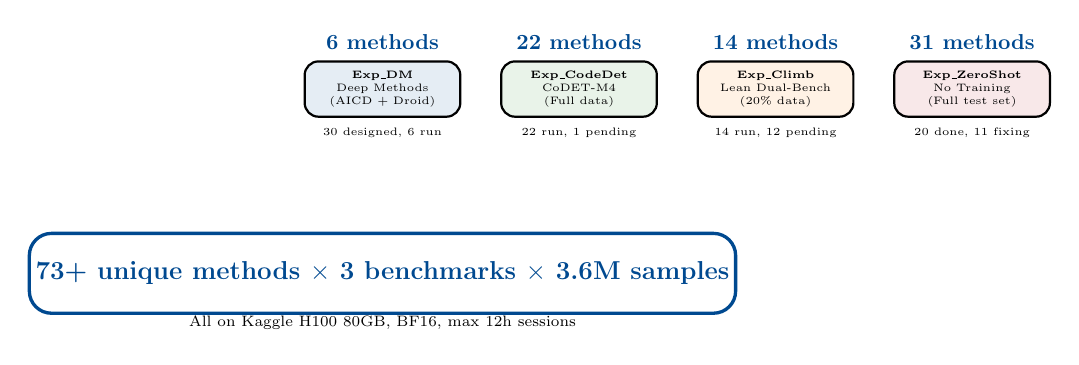
\begin{tikzpicture}[
    scale=0.78, transform shape,
    box/.style={draw, rounded corners=5pt, thick, font=\tiny, minimum height=0.9cm, minimum width=2.5cm, text width=2.3cm, align=center},
    bignum/.style={font=\normalsize\bfseries, mainblue}
]
    \node[box, fill=mainblue!10] (dm) at (0, 0) {\textbf{Exp\_DM}\\Deep Methods\\(AICD + Droid)};
    \node[bignum, above=0.05cm of dm] {6 methods};
    \node[font=\tiny, below=0.05cm of dm] {30 designed, 6 run};

    \node[box, fill=softgreen!10] (cd) at (3.2, 0) {\textbf{Exp\_CodeDet}\\CoDET-M4\\(Full data)};
    \node[bignum, above=0.05cm of cd] {22 methods};
    \node[font=\tiny, below=0.05cm of cd] {22 run, 1 pending};

    \node[box, fill=orange!10] (cl) at (6.4, 0) {\textbf{Exp\_Climb}\\Lean Dual-Bench\\(20\% data)};
    \node[bignum, above=0.05cm of cl] {14 methods};
    \node[font=\tiny, below=0.05cm of cl] {14 run, 12 pending};

    \node[box, fill=accentred!10] (zs) at (9.6, 0) {\textbf{Exp\_ZeroShot}\\No Training\\(Full test set)};
    \node[bignum, above=0.05cm of zs] {31 methods};
    \node[font=\tiny, below=0.05cm of zs] {20 done, 11 fixing};

    \node[draw, very thick, mainblue, rounded corners=8pt, minimum width=11.5cm, minimum height=1.3cm, yshift=-3cm] (total) {};
    \node[font=\large\bfseries, mainblue] at (total.center) {73+ unique methods $\times$ 3 benchmarks $\times$ 3.6M samples};
    \node[font=\scriptsize, below=-0.1cm of total] {All on Kaggle H100 80GB, BF16, max 12h sessions};
\end{tikzpicture}
\end{center}
\end{frame}


\begin{frame}{Updated Evaluation Matrix}
\vspace{-0.2cm}
\begin{center}\footnotesize
\renewcommand{\arraystretch}{1.1}
\begin{tabular}{@{}p{2.2cm}p{3.8cm}p{3.8cm}p{3.8cm}@{}}
\toprule
& \textbf{CoDET-M4} {\tiny ACL'25} & \textbf{DROID} {\tiny EMNLP'25} & \textbf{AICD} {\tiny EACL'26} \\
\midrule
\textbf{Binary} & \textcolor{softgreen}{\ding{51}} 99.09\% (RAG/MoE/KAN) & \textcolor{softgreen}{\ding{51}} 89.41\% T3 & \textcolor{orange}{\faClock} 30.88\% T1 (collapse) \\
\textbf{Attribution} & \textcolor{softgreen}{\ding{51}} \textbf{71.53\%} (6-cls) $\uparrow$ & --- & \textcolor{orange}{\faClock} 20.71\% T2 \\
\textbf{Refined} & --- & \textcolor{softgreen}{\ding{51}} 89.41\% T3 & \textcolor{orange}{\faClock} 57.06\% T3 \\
\textbf{Adversarial} & --- & \textcolor{softgreen}{\ding{51}} 88.02\% T4 & \textcolor{orange}{\faClock} T3 (hybrid) \\
\textbf{OOD Lang} & \textcolor{softgreen}{\ding{51}} 74.82\% avg $\uparrow$ & --- & \textcolor{orange}{\faClock} 3$\to$9 lang \\
\textbf{OOD Source} & \textcolor{softgreen}{\ding{51}} \textbf{55.42\%} (parity!) $\uparrow$ & --- & --- \\
\textbf{OOD Generator} & \textcolor{softgreen}{\ding{51}} 94.72\% W-F1 $\uparrow$ & --- & --- \\
\textbf{Zero-Shot} & \textcolor{softgreen}{\ding{51}} 31 methods $\uparrow$ & \textcolor{softgreen}{\ding{51}} 31 methods $\uparrow$ & --- \\
\bottomrule
\end{tabular}
\end{center}

\vspace{0.1cm}
{\small \textcolor{softgreen}{\ding{51}} = completed (with numbers). \textcolor{orange}{\faClock} = ongoing / challenging. $\uparrow$ = new since last report.}

\vspace{0.1cm}
\centering
\fbox{\parbox{0.85\textwidth}{\centering\small
\textbf{Progress since last report:}\\
Author F1: 70.55 $\to$ \textbf{71.53} (+0.98) | 22 methods on CoDET (was 10) | Full OOD suite done\\
Lean dual-bench: 14 methods | Zero-shot: 31 methods | Total: 73+ methods}}
\end{frame}


% ════════════════════════════════════════════════════════════════════════
\section{Next Steps}
% ════════════════════════════════════════════════════════════════════════

\begin{frame}{Next Steps \& Priorities}
\vspace{-0.25cm}
\begin{columns}[T]
\column{0.48\textwidth}
\begin{block}{\faRocket\ High Priority}
\scriptsize
\begin{enumerate}\setlength\itemsep{2pt}
    \item \textbf{DFR-SourceBalanced}: Last-layer retrain on balanced data. Target: OOD-GH $>$ 0.40
    \item \textbf{HierNCoE}: Hierarchical Neural Collapse + ETF. Target: Qwen F1 $\geq$ 0.50
    \item \textbf{FrontDoor-NLP}: Causal mediation for OOD-source
    \item \textbf{Full data training}: Scale 100K $\to$ 500K/1M
\end{enumerate}
\end{block}

\vspace{-0.1cm}
\begin{exampleblock}{\scriptsize Kill Criteria}
\tiny
A method is worth promoting iff it beats:\\
$\bullet$ CoDET Author $>$ 71.53 \textbf{OR}
$\bullet$ Droid T3 $>$ 89.41 \textbf{OR}\\
$\bullet$ OOD-SRC-gh $>$ 35.56 \textbf{OR}
$\bullet$ AICD T1 $>$ 0.31
\end{exampleblock}

\column{0.48\textwidth}
\begin{block}{\faPen\ Paper Writing}
\scriptsize
\begin{itemize}\setlength\itemsep{2pt}
    \item \textbf{NeurIPS 2026} target (deadline: October)
    \item Headline: ``20\% data + dual-bench SOTA''
    \item 3-benchmark evaluation (3.6M samples)
    \item 73+ method ablation = comprehensive study
    \item Zero-shot suite = separate appendix / paper
\end{itemize}
\end{block}

\vspace{-0.1cm}
\begin{alertblock}{\faClock\ Timeline}
\scriptsize
\begin{tabular}{@{}ll@{}}
Apr--May & Remaining Climb \& DM exps \\
Jun--Jul & Full data scaling + ablations \\
Aug--Sep & Paper writing + submission \\
Oct & NeurIPS 2026 deadline \\
\end{tabular}
\end{alertblock}
\end{columns}
\end{frame}


\begin{frame}{}
\vspace{1.5cm}
\begin{center}
{\Huge \textbf{Thank You}}
\vspace{0.8cm}

{\Large Questions \& Discussion}
\vspace{1cm}

{\small
\faDatabase\ CoDET-M4 {\tiny(ACL'25)} $\cdot$ DroidCollection {\tiny(EMNLP'25)} $\cdot$ AICDBench {\tiny(EACL'26)} \\[4pt]
\faStar\ \textbf{73+ methods} $\cdot$ \textbf{4 experiment suites} $\cdot$ \textbf{3.6M samples}
}
\end{center}
\end{frame}

\end{document}
